\chapter{Preliminary Analysis of a Rocket}
The following chapter describes the functionality and structure behind a rocket. The goal is to determine which factors that leads to instability in flight and launch of a rocket. 
\bigbreak

The rocket which will described is based on:
\begin{itemize}[noitemsep]
\item A payload system.
\item A guidance system to control the rocket.
\item A propulsion system to launch the rocket with. 
\item Structure system consisting of nose cone, frame and fins.
\end{itemize}    

\begin{figure}[htbp]
	\centering
 	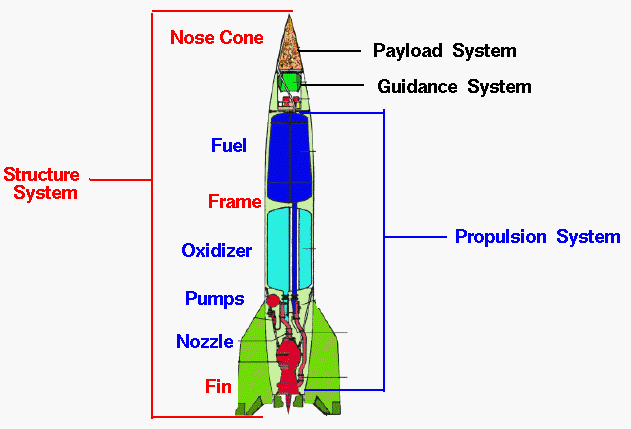
\includegraphics[width=0.7\textwidth]{figures/RocketStructure.png} 
 	\caption{Basic structure of a rocket.}
 	\label{fig:RocketStructure}
\end{figure}
%https://spaceflightsystems.grc.nasa.gov/education/rocket/rockpart.html

%Rocket stability page
\subsection{Controlling a Rocket's Stability}
The design method for placing the CP and GP does not always provide a perfectly stable attitude control. Indeed to have such precision an active control system is necessary. Full scale rockets use the thrusting force to achieve alike control. In order to do so most of them operate with the gimbaled thrust method. It consists of steering the engine's nozzle to get the thrusting force in right incidence. An example is seen cf. figure \autoref{fig:RocketGimbal}. 
\begin{figure} [htbp]
	\centering
	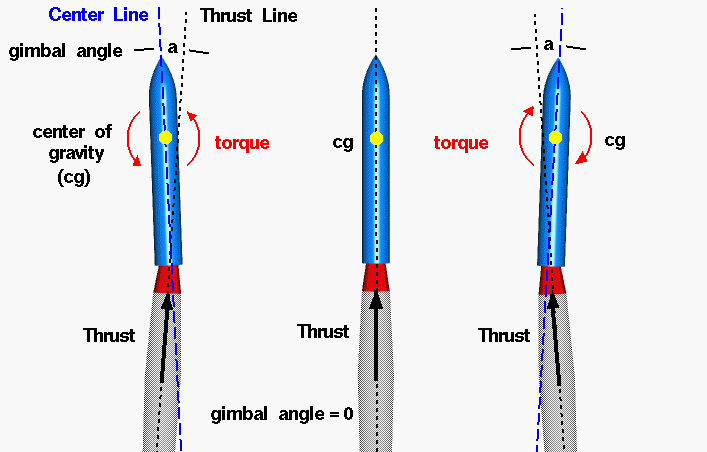
\includegraphics[width=0.8\linewidth]{RocketGimbal}
	\caption{Example of gimballing a rocket nozzle \cite{web:rocketnasa}.}
	\label{fig:RocketGimbal}
\end{figure}
\newpage

Where a torque is applied to create a rotation around the rocket's center of gravity. The thrust direction is relative to the position of the center of gravity.  This should compensate for direction deviations from the rocket's center line or trajectory, and keep the rocket stable. The described gimbal method will be the control method focused on in this project. The rocket will be designed with a control system depending on vectoring the thruster in relation to the attitude position of the rocket. 



\section{Mechanical System of a Rocket}
Input/output relation of a rocket.
\section{The Inverse Pendulum}
relate the rocket model to a Inverse Pendulum